\documentclass[../main]{subfiles}

\begin{document}

\section{Functions and Linear Graphs}

\subsection{Cartesian Coordinates}

The \textbf{Cartesian coordinate system} describes the positions of points and
lines in a plane. A Cartesian plane consists of a horizontal axis and a vertical
axis.
\begin{enumerate}
\item The horizontal axis: \textbf{x-axis}
\item  The vertical axis: \textbf{y-axis}
\item The two axes intersect at the origin, \(O\).

\end{enumerate}

The position of any point on the Cartesian plane is represented as an ordered
pair \((a,b)\) of real numbers know as \textbf{coordinates}.

Note:
\(a\) is know as the \(x-coordinate\)
\(b\) is know as the \(y-coordinate\)

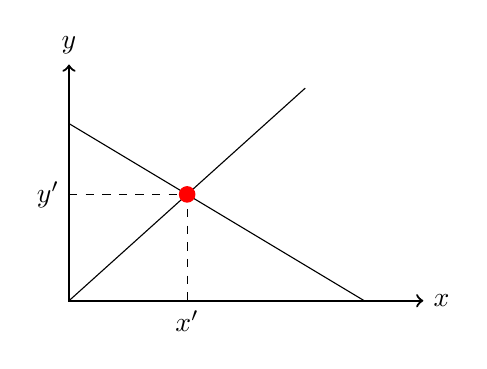
\begin{tikzpicture}[scale=1.5]
    % Draw axes
    \draw [<->,thick] (0,2) node (yaxis) [above] {$y$}
        |- (3,0) node (xaxis) [right] {$x$};
    % Draw two intersecting lines
    \draw (0,0) coordinate (a_1) -- (2,1.8) coordinate (a_2);
    \draw (0,1.5) coordinate (b_1) -- (2.5,0) coordinate (b_2);
    % Calculate the intersection of the lines a_1 -- a_2 and b_1 -- b_2
    % and store the coordinate in c.
    \coordinate (c) at (intersection of a_1--a_2 and b_1--b_2);
    % Draw lines indicating intersection with y and x axis. Here we use
    % the perpendicular coordinate system
    \draw[dashed] (yaxis |- c) node[left] {$y'$}
        -| (xaxis -| c) node[below] {$x'$};
    % Draw a dot to indicate intersection point
    \fill[red] (c) circle (2pt);
\end{tikzpicture}
\end{document}